\section{JavaScript}
\label{sec:javascript}
JavaScript é uma linguagem de programação adotada amplamente pela maioria das páginas \textit{web}, além de ser utilizada também em outros ambientes fora do navegador através de tecnologias auxiliares. Trata-se de uma linguagem interpretada, originalmente implementada diretamente como parte dos navegadores \textit{web} para que os scripts pudessem ser executados \textit{client-side} sem a necessidade de passar por um servidor \cite{Mozilla2023}.

JavaScript é baseado em protótipos, leve, dinâmico e \textit{single-thread}, dando suporte a vários paradigmas de programação diferentes, como a programação orientada a objetos, a imperativa e a declarativa. Além disso, diferencia-se também por utilizar o tipo de compilação \textit{just-in-time}, compilando seu código durante a sua execução \cite{Mozilla2023}.

\begin{figure}[H]
    \centering
    \caption{Código exemplo em JavaScript.}
    \label{fig:javascript}
    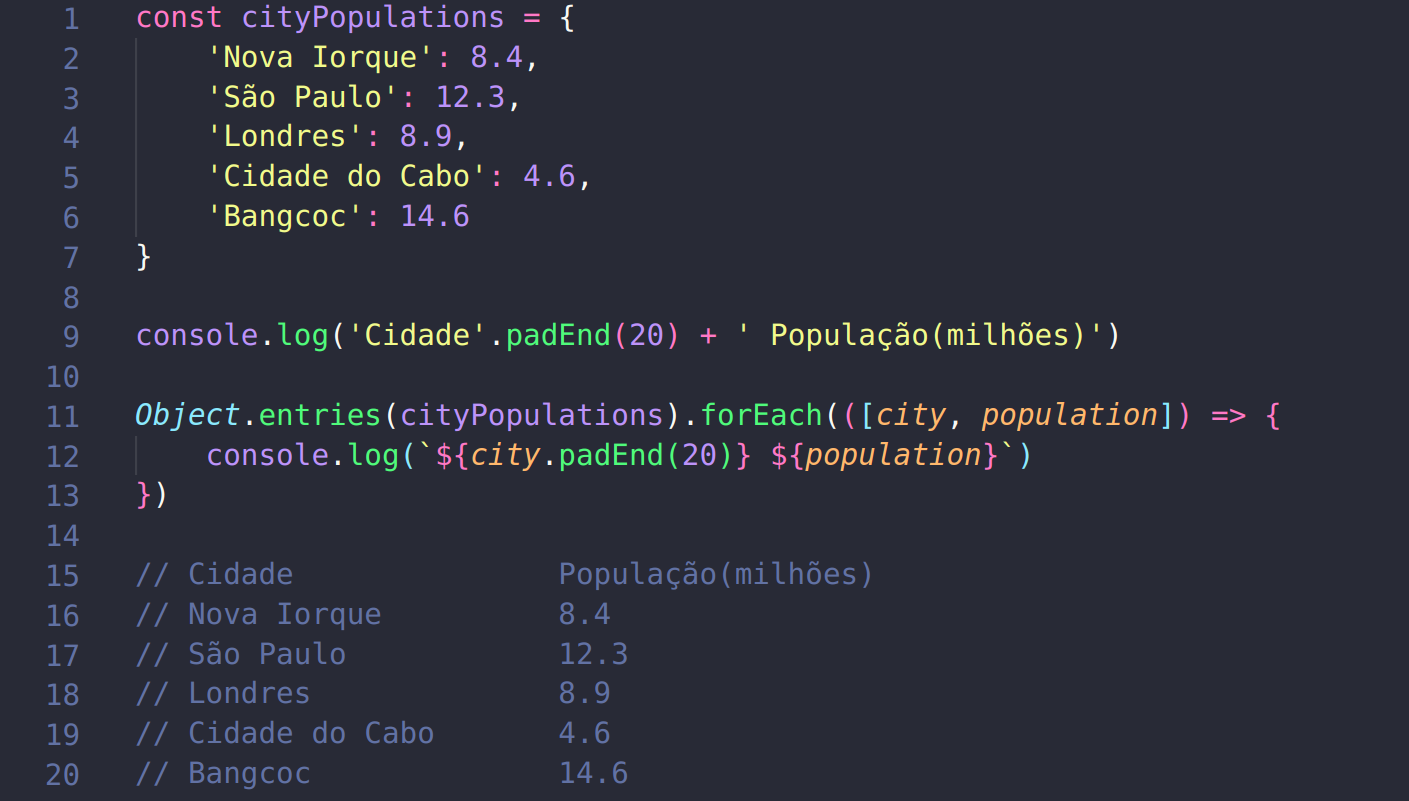
\includegraphics[width=.65\textwidth]{data/figures/javascript.png}
    \fonte{Autor}
\end{figure}

A linguagem foi criada em 1995 principalmente pelo programador Brendan Eich a pedido da empresa NetScape para lidar com a validação de formulários HTML. Para que a linguagem evoluísse obedecendo padronizações já estabelecidas no mercado, os criadores da linguagem associaram-se à fundação ECMA um ano após sua criação, entretanto, o nome JavaScript já havia sido patenteado, decidindo-se seguir pelo nome oficial de ECMAScript.

Todavia, de acordo com \citeonline{Malavasi2017}, na comunidade de desenvolvedores a linguagem ainda é chamada de JavaScript até os dias atuais, utilizando o nome oficial ECMAScript apenas para referenciar suas versões.